\documentclass[11pt,spanish]{article} % Idioma
\usepackage{babel}
\usepackage[T1]{fontenc}
\usepackage{textcomp, verbatim} % \begin{comment}
\usepackage[utf8]{inputenc} % Permite acentos

\usepackage{wrapfig} % Imagenes %\graphicspath{ {./imagenes/} }
\usepackage[left=2.75cm,top=2.5cm,right=2cm,bottom=2.5cm]{geometry} % Márgenes
\usepackage{amssymb, amsmath, amscd, amsfonts, amsthm, mathrsfs } % Símbolos matemáticos
\usepackage{cancel} % Cancelar expresiones
\usepackage{multirow, multicol, tabularx, booktabs, longtable} % Tablas
\usepackage{fancyhdr, fncychap} % Encabezados
\usepackage{algpseudocode, algorithmicx, algorithm} % Pseudo-código
\usepackage{bbding} % Símbolos
\usepackage{enumitem} % Enumerados a), b), c)... usando \begin{enumerate}[label=\alph*)]
\usepackage{graphicx, xcolor, color, pstricks} % Gráficos --TikZ--
% http://www.texample.net/tikz/examples/
\usepackage[hidelinks]{hyperref}  % Enlaces
\usepackage{verbatim} % Comentarios largos \begin{comment}
\usepackage{rotating} % \begin{rotate}{30}
\usepackage[all]{xy} % Diagramas
\usepackage{listings} % Escribir código
\usepackage{xparse} % Entornos



\usepackage[nottoc]{tocbibind} % Incluir bibliografía en el índice


\usepackage{hyperref}
\hypersetup{
	colorlinks=true,
	linkcolor=black,
	filecolor=magenta,
	urlcolor=cyan,
}



% Comandos
\newcommand{\docdate}{}
\newcommand{\subject}{}
\newcommand{\docauthor}{Rubén Morales Pérez}
\newcommand{\docemail}{srmorales@correo.ugr.es}

\newcommand{\N}{\mathbb{N}}
\newcommand{\Q}{\mathbb{Q}}
\newcommand{\C}{\mathbb{C}}
\newcommand{\R}{\mathbb{R}}
\newcommand{\Z}{\mathbb{Z}}


\linespread{1.1}                  % Espacio entre líneas.
\setlength\parindent{0pt}         % Indentación para párrafo.

\title{Prácticas Fundamentos de Redes \\ Chromecast}
\author{Francisco Javier Morales Piqueras \\
		María Florencio Díaz\\
		Rubén Morales Pérez}
\date{\today}

% % % % % % % % % % % % % % % % % % % % % % % % % % % % % % % % %
%					 Inicio del documento
% % % % % % % % % % % % % % % % % % % % % % % % % % % % % % % % %
\begin{document}

\maketitle
\tableofcontents % Generando el indice
\newpage



\section{Introducción}
Google Chromecast es un dispositivo de reproducción multimedia fabricado por Google y comercializado a partir de Julio de 2013. Reproduce contenido multimedia conectado a una televisión o monitor vía HDMI haciendo streaming mediante Wi-Fi. Un nuevo modelo Chromecast Ultra que soporta 4k fue anunciado durante el evento \#MadeByGoogle.

\

Para hacer streaming utiliza el software Google Cast, un protocolo propietario de Google que permite controlar la reproducción de contenido multimedia desde un dispositivo local en otro dispositivo compatible con esta tecnología. Google Cast dispone de librerías para las últimas versiones de Android y iOS, así como para Chrome OS y aplicaciones de Google Chrome.

\begin{figure*}[h]
	\centering
	\begin{minipage}[b]{.35\textwidth}
		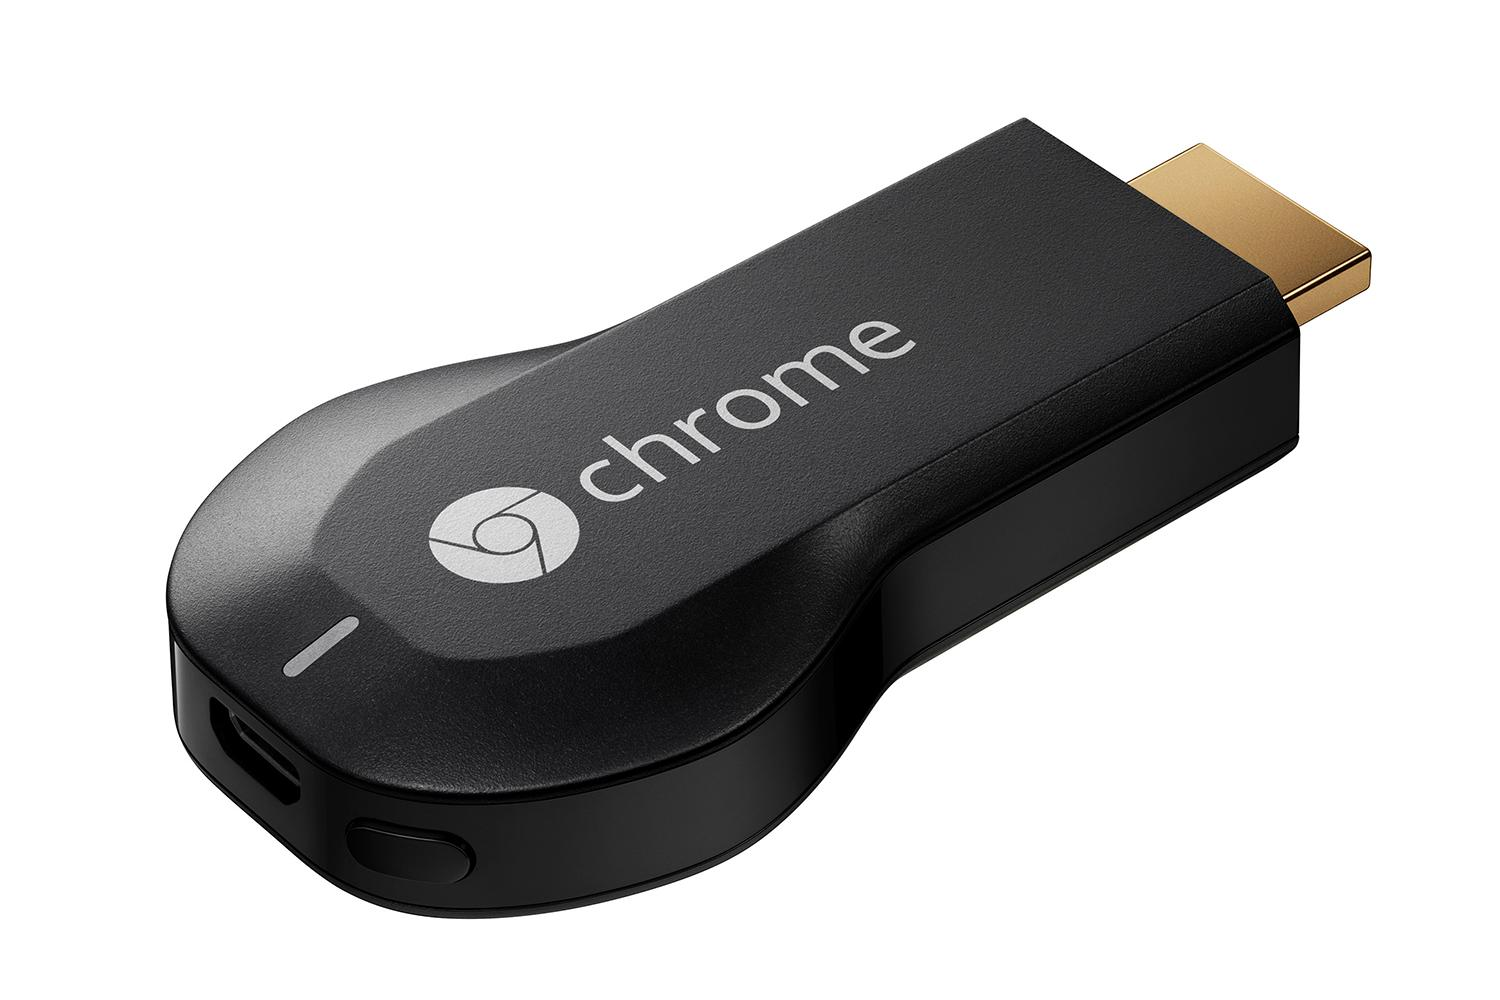
\includegraphics[scale=0.11]{./Imagenes/chromecast1gen.jpg}
		\caption{Primera generación}\label{fig:1gen}
	\end{minipage}\qquad
	\hspace{1cm}
	\begin{minipage}[b]{.35\textwidth}
		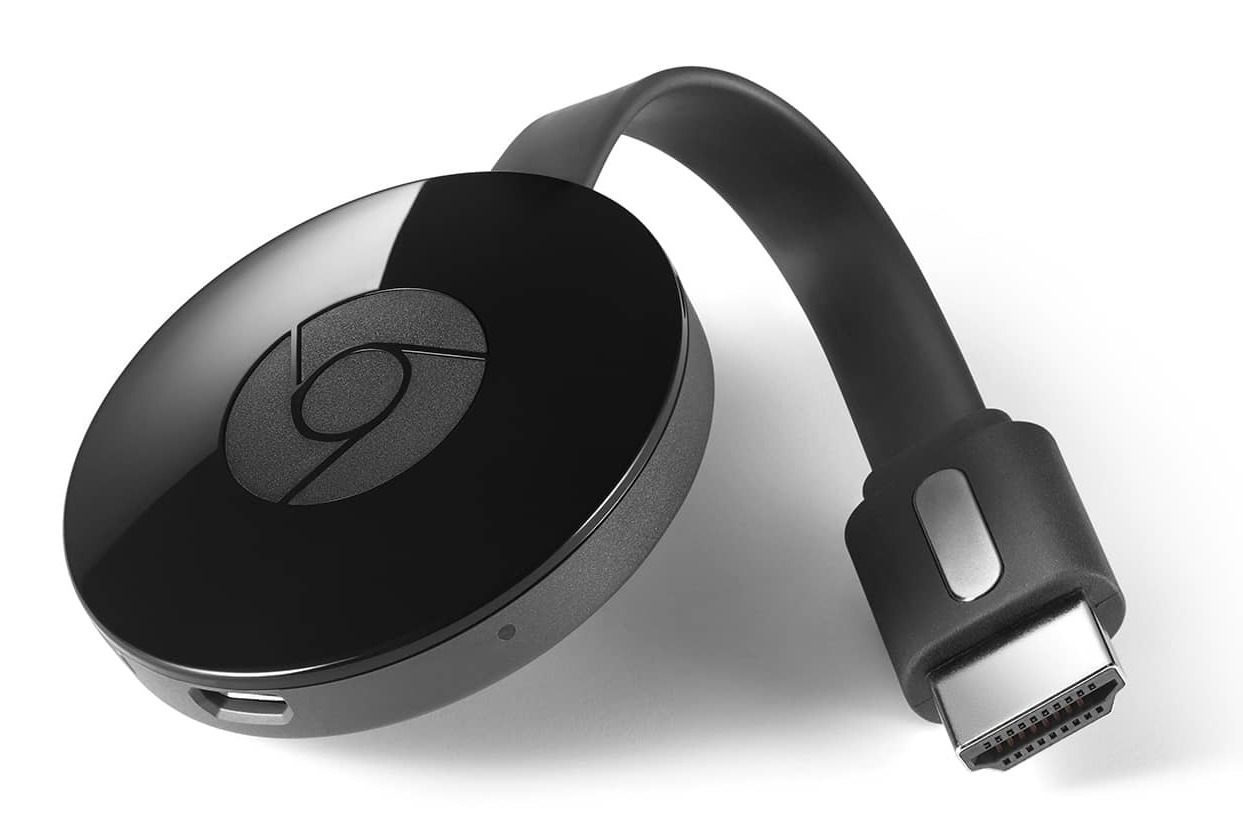
\includegraphics[scale=0.15]{./Imagenes/Chromecast.jpg}
		\caption{Segunda generación}\label{fig:2gen}
	\end{minipage}
\end{figure*}

Chromecast permite reproducir contenido almacenado en un dispositivo conectado a la red local o en un sevidor externo. El control de la reproducción se realiza en ambos casos desde uno o varios dispositivos locales compatibles con la tecnología Google Cast.

\

Cuando no hay contenido en streaming reproduce un contenido personalizable de fondo, puede incluir fotos personales,
de satélite, noticias, etc. Por defecto muestra imágenes aleatorias seleccionadas por Google.

\

Su principal competidor es el servicio AirPlay desarrollado por Apple, que permite streaming inalámbrico entre dispositivos iPhone, iPad o Mac para audio, vídeo, fotos, etc.

\vspace{1cm}
\begin{figure}[h]
	\centering
	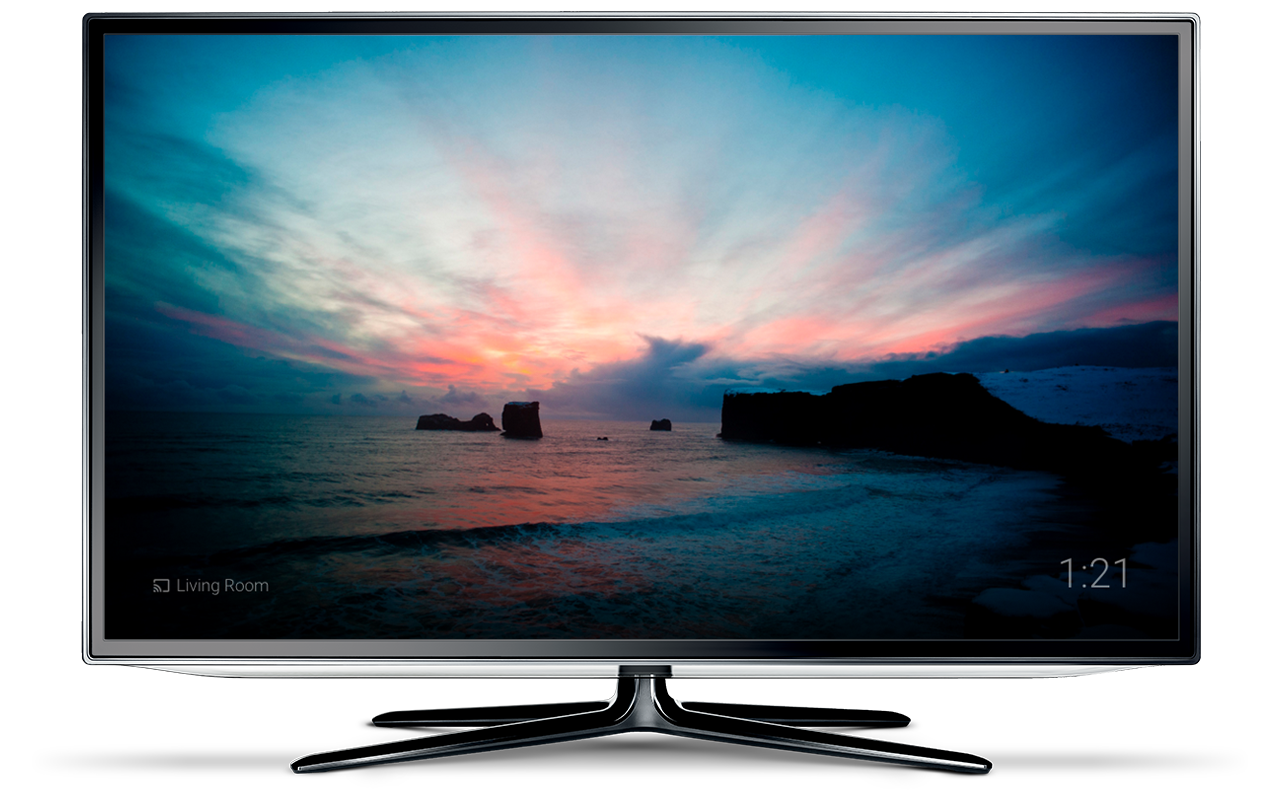
\includegraphics[width=0.6\textwidth]{./Imagenes/fondo.png}
	\label{fig:fondo}
\end{figure}

\newpage


\subsection{Generaciones}

El chromecast de primera generación incluye un decodificador de VP8 y H.264 para formatos de compresión de vídeo, 512 MB de Micron DDR3L RAM y 2 GB de memoria flash.
El de segunda generación tiene un cable flexible y magnético, usa procesador dual ARM Cortex-A7 de frecuencia 1.2 GHz y tiene tres antenas adaptativas para mejroar la conexión con el router.
El dispositivo tiene 512 MB de Samsung DDR3L RAM y 256 MB de memoria flash.

\section{Hardware}

\begin{figure}[h]
	\centering
	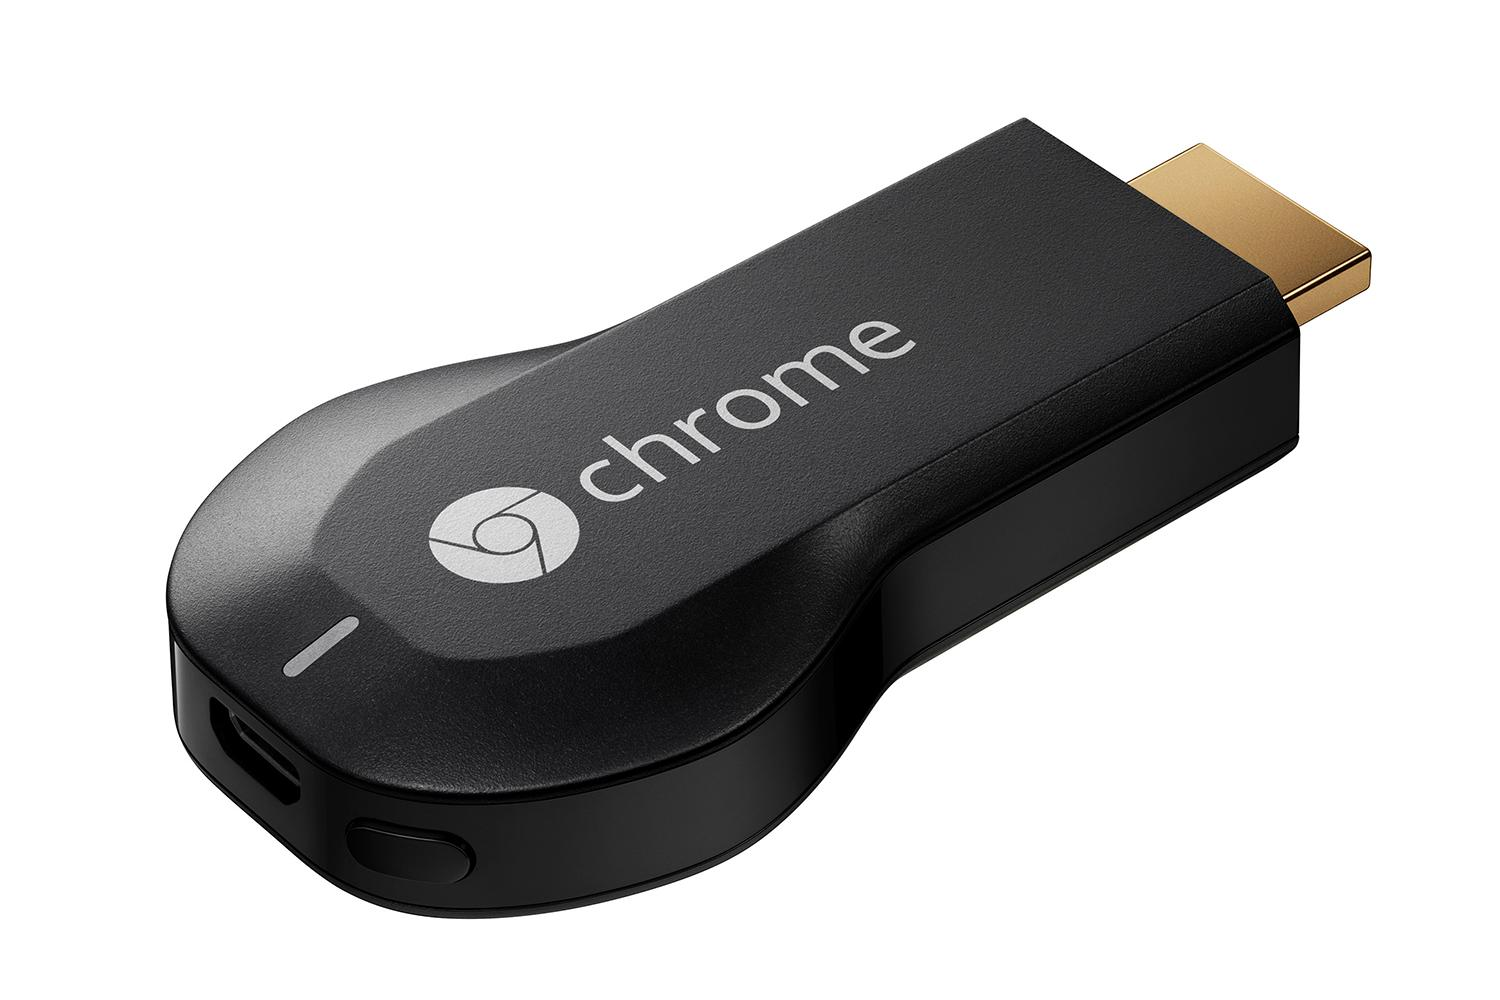
\includegraphics[width=0.45\textwidth]{./Imagenes/chromecast1gen.jpg}
	\caption{Chromecast de primera generación}\label{fig:1gen}
\end{figure}

El Chromecast de primera generación incluye un decodificador de VP8 y H.264 para formatos de compresión de vídeo, 512 MB de Micron DDR3L RAM y 2 GB o 4 GB de memoria flash según la fuente (Google no ha publicado las especificaciones del dispositvo).
Se conoce que tiene un chip a 700 MHz single core.
Tiene una salida HDMI, una entrada micro USB para la alimentación, un LED que indica el estado del dispositivo y un botón de reset.
Sus estándares de conexión son Wi-Fi 802.11 b/g/n (solo 802.11n a 2,4 GHz).

\

El de segunda generación tiene 512 MB de Samsung DDR3L RAM y 256 MB de memoria flash.
El dispositivo tiene un cable flexible en cuyo extremo se encuentra la salida HDMI, usa un procesador dual core ARM Cortex-A7 con 1.3 GHz de frecuencia y tiene tres antenas adaptativas para mejorar la conexión con el router.
Sus estándares de conexión son 802.11 b/g/n/ac Wi-Fi (2,4 GHz/5 GHz).

\begin{figure}[h]
	\centering
	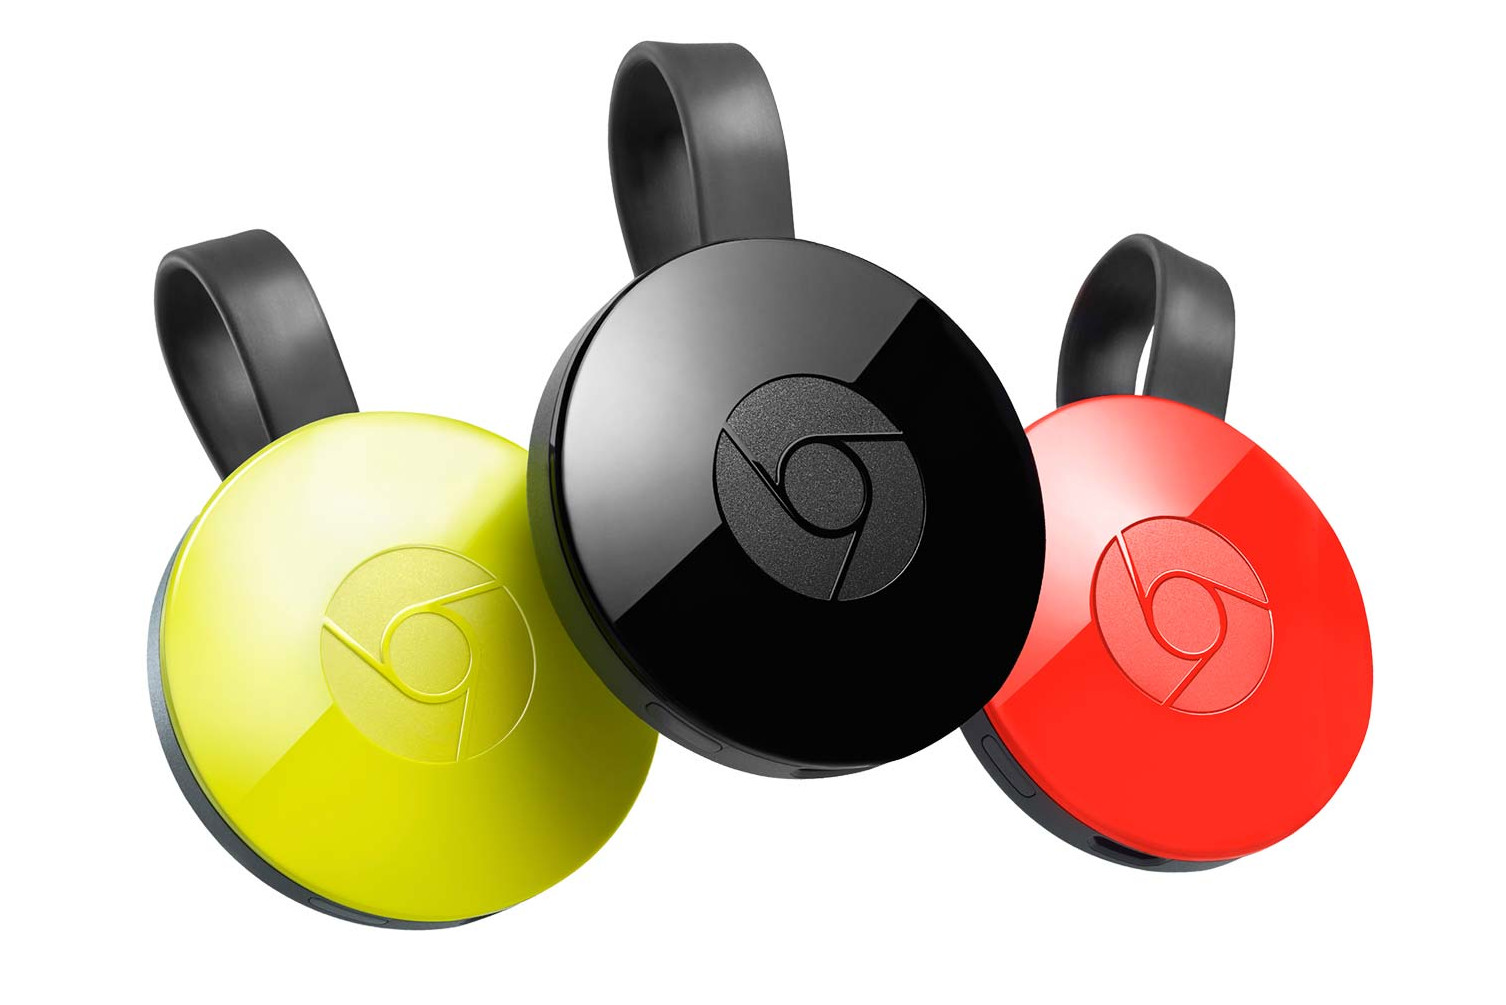
\includegraphics[width=0.55\textwidth]{./Imagenes/chromecast2gen.jpg}
	\caption{Chromecast de segunda generación}\label{fig:2gen}
\end{figure}

El Chromecast Audio es externamente igual que el de segunda generación, pero tiene una salida Minijack de 3,5mm en lugar del HDMI y un chip de procesamiento de audio.

\begin{figure}[h]
	\centering
	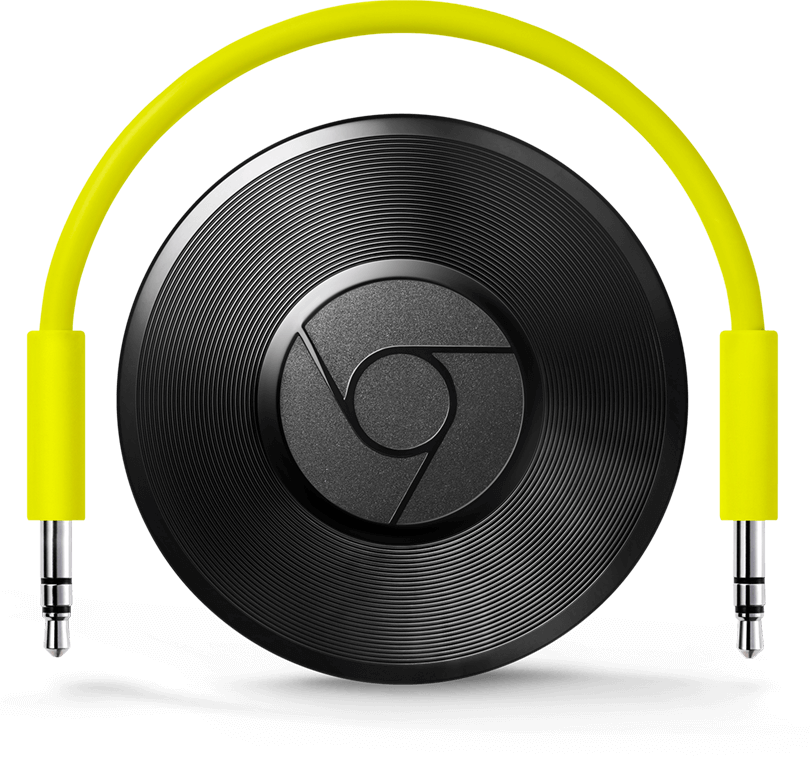
\includegraphics[width=0.4\textwidth]{./Imagenes/chromecastaudio.png}
	\caption{Chromecast Audio}\label{fig:audio}
\end{figure}

Acerca del hardware del Chromecast Ultra se conoce poco de manera oficial.
La mayor diferencia es, aparte de mayor potencia de procesamiento para reproducir vídeo 4K, una entrada Ethernet en el adaptador de corriente para conectarlo a Internet como alternativa al Wi-Fi.

\begin{figure}[h]
	\centering
	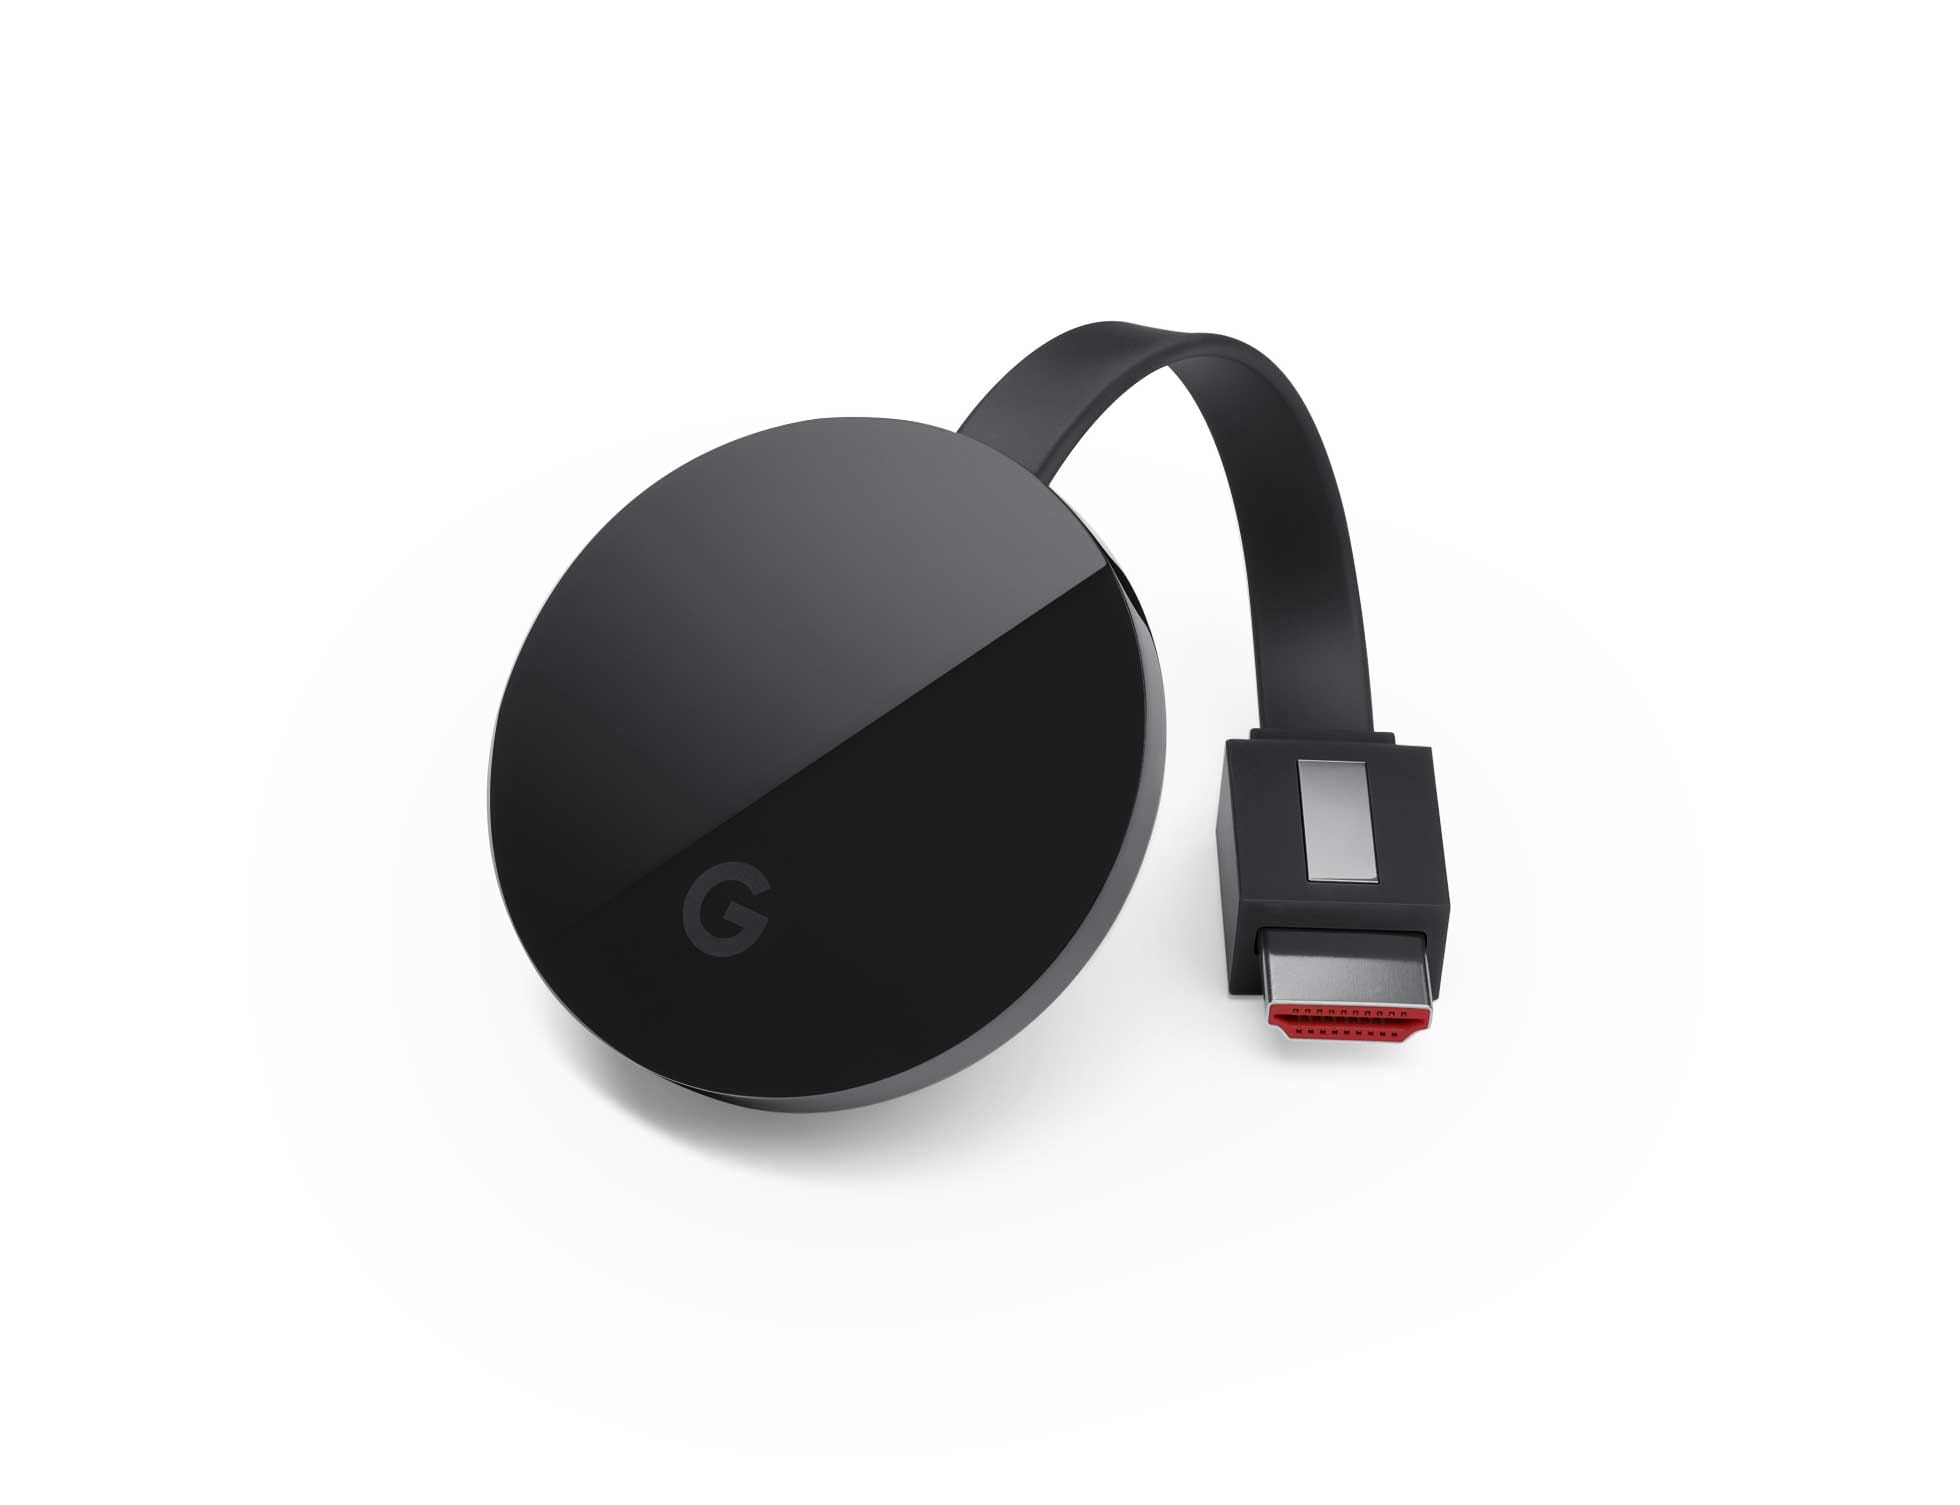
\includegraphics[width=0.42\textwidth]{./Imagenes/chromecast-ultra.jpg}
	\caption{Chromecast Ultra}\label{fig:ultra}
\end{figure}

\section{Software}

EL Google Chromecast no es más que un dispositivo compatible con el protocolo propietario de Google Cast que actúa como receptor.
Este protocolo fue lanzado en julio de 2013 en exclusividad para las aplicaciones de YouTube, Google Play Music, Google Play Movies & TV y Netflix usando como receptor el Chromecast de primera generación, pero en febrero de 2014 pusieron el SDK a disposición de todos los desarrolladores para usarlo en sus propias aplicaciones.
En mayo de 2015 había más de 20.000 aplicaciones de terceros compatibles con esta tecnología según reconoce Google.

\

Para iniciar la reproducción de un contenido pulsamos el botón de \textit{cast}, que aparecerá automáticamente si Google Cast está integrado con la aplicación.
En ese momento aparecen los dispositivos Chromecast conectados a la red local y se elige aquel donde se quiere emitir el contenido.
Si el puerto HDMI dispone de Consumer Electronics Control (CEC) la televisión se encenderá inmediatamente.

\

Google Cast tiene dos modos de funcionamiento:

\begin{itemize}

	\item Uno es usar dispositivo desde el que solicitamos el streaming para controlar la reproducción (en adelante dispositivo emisor): pausar un vídeo, subir el volumen del audio, crear o modificar una cola de reproducción, etc.
	El dispositivo receptor (por ejemplo un Chromecast) es quien se encarga de descargarlo y comunicarse con el servidor de contenido, liberando al dispositivo emisor de esta tarea.
	Esto garantiza una carga de trabajo muy baja para el emisor y le permite estar bloqueado mientras la reproducción está teniendo lugar.
	El contenido puede estar almacenado localmente en el dispositivo emisor o en un servidor externo.
	El primer caso ocurre en aplicaciones como Google Photos, mientras que un ejemplo del segundo serían Netflix o YouTube.
	Las aplicaciones emisoras que usen este modo de funcionamiento deben ser compatible con Android 4.1, iOS 7.0 o versiones superiores si son aplicaciones móviles y con Windows 7, macOS 10.7, Chrome OS 28 o versiones superiores si son aplicaciones Chrome.
	En este último caso, se debe tener instalada la extensión Cast.

	\item El otro modo es hacer mirroring de una pestaña de Chrome o del escritorio de un ordenador con Chrome o del de un dispositivo con Android 4.4 o superior.
	La calidad del streaming en este caso varía ampliamente según la potencia de procesamiento del emisor.
	En el caso de hacerse desde un smartphone, la calidad de las imágenes normalmente se deteriora debido al escalado.

\end{itemize}

Hasta diciembre de 2014, el dispositivo emisor y receptor debían estar conectados a la misma red Wi-Fi para reproducir contenido, pero en las versiones posteriores a esa fecha ya no es necesario.
Esto se debe a que se ha añadido un modo invitado.
En este modo, el receptor emite ultrasonidos a través de los altavoces y el emisor es capaz de localizarlo usando el micrófono.
Se usa un PIN de cuatro dígitos que aparece en pantalla para la verificación.
El modo invitado está disponible para todos los Chromecast con un dispositivo Android como emisor y para los Chromecast a partir de la segunda generación para aquellos con dispositivos iOS como emisor.

\

Como hemos adelantado, la API de Google Cast implementa el paradigma del productor-consumidor. Para implementar el protocolo hacen falta dos aplicaciones:

\begin{itemize}

	\item La aplicación emisora que se encarga de proveer al usuario la capacidad de controlar la reproducción y elegir el dispositivo donde se emite el contenido.
	Esta aplicación crea un canal seguro con la aplicación receptura para el intercambio de mensajes.

	\item La aplicación receptora es una web app ejecutándose en una versión adaptada del navegador Chrome con una interfaz gráfica en CSS.
	La aplicación receptora puede tener una complejidad muy variable, pudiendo ir desde limitarse a reproducir contenido HTML5 hasta soportar protocolos de streaming como MPEG-DASH, HTTP Live Streaming o el Microsoft Smooth Streaming Protocol\cite{DLNA-Miracast}.

\end{itemize}

Los formatos multimedia a los que Google Cast da soporte son los siguientes:

\begin{itemize}

	\item Imágenes en formato BMP, GIF, JPEG, PNG y WEBP, con un límite de 1280x720 píxeles de resolución.

	\item Los codecs de audio HE-AAC, LC-AAC, MP3, Vorbis, WAV (LPCM) y FLAC. AC-3 (Dolby Digital) y E-AC-3 (EC-3, Dolby Digital Plus) están disponibles para passthrough de audio.

	\item Los codecs de vídeo H.264 High Profile Level 4.1 (decodificación hasta 720/60 o 1080/30) y VP8.

\end{itemize}

Chromecast para buscar dispositivos disponibles en una red Wi-Fi usa el protocolo mDNS (multicast Domain Name System), anteriormente usaba el protocolo DIAL (DIscovery And Launch).

Para la visualización de contenidos en la TV se mezclan conceptos DLNA (Digital Living Network Alliance) y Miracast\cite{DLNA-Miracast}.
A la hora de enviar contenido realmente se manda la orden a Chromecast de que reproduzca el contenido elegido directamente desde la nube.
Es la principal diferencia con DLNA, ya que no se reproduce contenido desde un servidor DLNA sino desde Internet.
Para usar solamente DLNA para streaming necesitaríamos aplicaciones de terceros, por ejemplo iMediaShare.
Otra funcionalidad es poder enviar los contenidos de una pestaña del navegador Chrome a la TV en lo que podríamos denominar una conexión Miracast pura y dura, punto a punto.




\begin{figure}[ht]
	\begin{minipage}[b]{0.55\linewidth}
	Utiliza un sistema operativo de escritorio llamado Chrome OS, siendo el navegador Google Chrome su principal herramienta de uso.
	Chrome OS se basa en el proyecto de código abierto Chromium OS,5 que, a diferencia de Chrome OS, se puede compilar a partir del código fuente descargado.
	\end{minipage}%%
	\begin{minipage}[b]{0.45\linewidth}
		\centering
		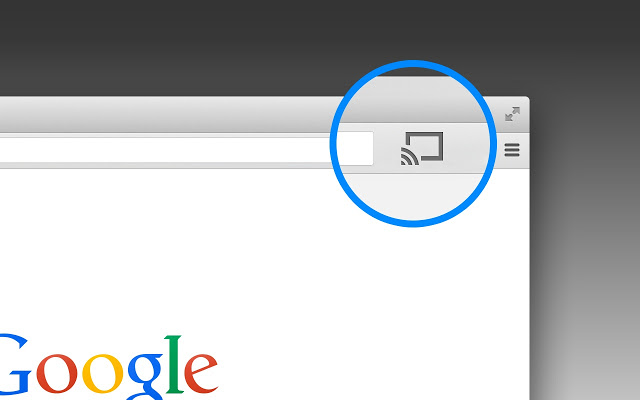
\includegraphics[width=.65\linewidth]{./Imagenes/googlecastbrowser.jpg}
	\end{minipage}
\end{figure}







\subsection{Google Cast}
\subsubsection{Google Home}

\subsection{mDNS (multicast Domain Name System)}


\subsection{Miracast}
Miracast es un protocolo multimedia para hacer streaming a un monitor desde un dispositivo local. Para que nuestra smartTV sea capaz de usarlo, necesita soportar Wi-Fi Direct. Wi-Fi Direct es una norma que permite la conexión entre dos dispositivos Wi-Fi sin necesidad de un intermediario.
Los dispositivos que envían y reciben información tienen que estar certificados para Miracast, pero existe un plug para dispositivos no certificados.
Miracast está disponible de manera nativa para dispositivos con versiones de Android 4.2 y Android 6.0.

\vspace{0.1cm}
\begin{figure}[ht]
	\begin{minipage}[b]{0.55\linewidth}
		La conexión está creada vía Wi-Fi Protected Setup (WPS), mecanismos para facilitar la configuración de una red WLAN con seguridad WPA2.
		WPS contempla cuatro configuraciones para el intercambio de credenciales: PIN (Personal Identification Number), PBC (Push Button Configuration), NFC (Near Field Communications) y USB (Universal Serial Bus). La configuración PIN no es recomendable por su debilidad ante ataques de fuerza bruta.
	\end{minipage}%%
	\begin{minipage}[b]{0.45\linewidth}
		\centering
		
\includegraphics[width=.55\linewidth]{./Imagenes/miracast.jpg}
	\end{minipage}
\end{figure}

\

Para la capa de internet usa IPv4; para la de transporte, TCP/UDP, y para la de aplicación, RTSP y RTP, que se encargan de controlar el streaming.

\

A partir de Android 6.0, Google ha dejado de dar soporte nativo a Miracast en favor de su propio Google Cast.
Con Miracast el dispositivo receptor es dependiente de que el dispositivo Android emisor se mantenga activo \cite{Miracast}: si se bloquea también bloqueará la reproducción en el receptor.
Esto implica una mayor carga de trabajo y consumo de batería respecto a Google Cast, que solo se encarga de enviar señales para el control de la reproducción.

\

Existe una alternativa de código abierto a Miracast llamada MiracleCast. El nombre viene por la dificultad de crear una red Wifi-P2P estable (basado en wpa_supplicant).

\

El núcleo de MiracleCast es un demonio llamado miracled \cite{MiracleCast}, que controla links locales, las peticiones de conexión, se encarga de la codificación del protocolo y el parsing.
Su línea de comandos puede ser usada para controlar el demonio, crear nuevas conexiones, modificar parámetros, etc.
Soporta un modo interactivo que muestra las peticiones de conexión y permite al usuario aceptarlas o no.

\

El código fuente se puede encontrar en \href{https://github.com/albfan/miraclecast}{github}.



\subsection{Chrome OS?}

\section{Aplicaciones}
En el primer lanzamiento YouTube y Netflix eran soportadas como aplicaciones web en Android, iOS, y navegador Chrome, Google Play Music y Google Play Movies $\&$ TV eran soportadas como aplicaciones.
El SDK estuvo abierto para desarrolladores a partir de Febrero de 2014, ahora es parte del framework de Google Play Services.

Una lista completa de las aplicaciones compatibles se puede encontrar en la 
\href{https://www.google.com/intl/en/chromecast/apps/}{página web de chromecast}





% % % % % % % % % % % % % % % % % % % % % % % % % % % % % % % % %
%					 Bibliografía
% % % % % % % % % % % % % % % % % % % % % % % % % % % % % % % % %


% Para hacer citas: \cite{<referencia>}
% donde <referencia> es lo primero que aparece en el fichero .bib:
% @tipo{<referencia>, ...}

% Si no se utiliza una cita hay que especificarlo con \nocite{<referencia>}


 % El orden de referencias es determinado por el orden de aparición de \cite y \nocite
\bibliographystyle{unsrt}

\bibliography{./Bibliografia/preambulo,./Bibliografia/referencias}


\end{document}
